%%%%%%%%%%%%%%%%%%%%%%%%%%%%%%%%%%%%%%%%%%%%%%%%%%%%%%%%%%%%%%%%%%%%%%%%%%%%%%%%%%
\begin{frame}[fragile]\frametitle{}
\begin{center}
{\Large Q Learning}
\end{center}
\end{frame}

%%%%%%%%%%%%%%%%%%%%%%%%%%%%%%%%%%%%%%%%%%%%%%%%%%%%%%%%%%%%%%%%%%%%%%%%%%%%%%%%%%
\begin{frame}[fragile]\frametitle{A Taxonomy of RL Algorithms}

\begin{center}
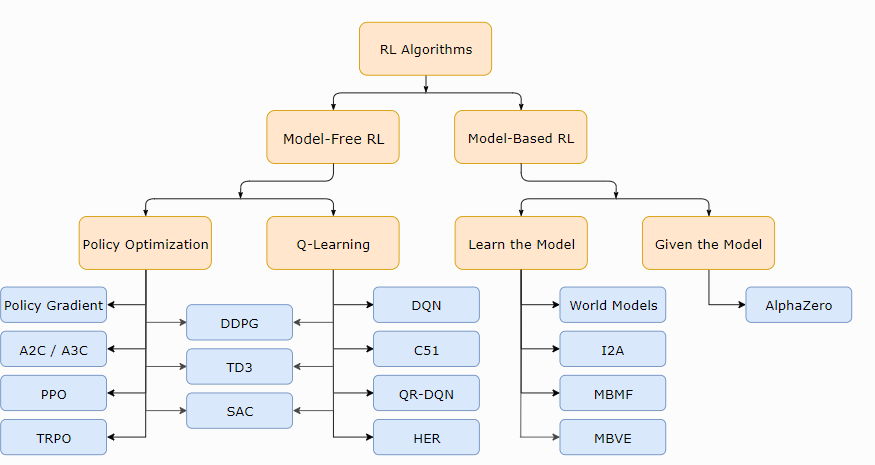
\includegraphics[width=\linewidth,keepaspectratio]{rl100}
\end{center}

{\tiny (Ref: Spinning Up - Open AI)}
\end{frame}

%%%%%%%%%%%%%%%%%%%%%%%%%%%%%%%%%%%%%%%%%%%%%%%%%%%%%%%%%%%%%%%%%%%%%%%%%%%%%%%%%%
\begin{frame}[fragile]\frametitle{Model-Free vs Model-Based RL}

\begin{itemize}
\item Core question: whether the agent has access to (or learns) a model of the environment. By a model of the environment, we mean a function which predicts state transitions and rewards.
\item Advantage of having model is that it allows the agent to plan by thinking ahead, seeing what would happen for a range of possible choices, and explicitly deciding between its options. Agents can then distill the results from planning ahead into a learned policy. A particularly famous example of this approach is AlphaZero. When this works, it can result in a substantial improvement in sample efficiency over methods that don’t have a model.
\item The main downside is that a ground-truth model of the environment is usually not available to the agent. 
\item If an agent wants to use a model in this case, it has to learn the model purely from experience, which creates several challenges. 

\end{itemize}

{\tiny (Ref: Spinning Up - Open AI)}
\end{frame}

%%%%%%%%%%%%%%%%%%%%%%%%%%%%%%%%%%%%%%%%%%%%%%%%%%%%%%%%%%%%%%%%%%%%%%%%%%%%%%%%%%
\begin{frame}[fragile]\frametitle{Model-Free vs Model-Based RL}

\begin{itemize}
\item The biggest challenge is that bias in the model can be exploited by the agent, resulting in an agent which performs well with respect to the learned model, but behaves sub-optimally (or super terribly) in the real environment. 
\item Model-learning is fundamentally hard, so even intense effort—being willing to throw lots of time and compute at it—can fail to pay off.
\item Algorithms which use a model are called model-based methods, and those that don’t are called model-free. 
\item While model-free methods forego the potential gains in sample efficiency from using a model, they tend to be easier to implement and tune.
\end{itemize}

{\tiny (Ref: Spinning Up - Open AI)}
\end{frame}

%%%%%%%%%%%%%%%%%%%%%%%%%%%%%%%%%%%%%%%%%%%%%%%%%%%%%%%%%%%%%%%%%%%%%%%%%%%%%%%%%%
\begin{frame}[fragile]\frametitle{What to Learn}

Another critical branching point in an RL algorithm is the question of what to learn. The list of usual suspects includes


\begin{itemize}
\item policies, either stochastic or deterministic,
\item action-value functions (Q-functions),
\item value functions,
\item and/or environment models.
\end{itemize}

{\tiny (Ref: Spinning Up - Open AI)}
\end{frame}

%%%%%%%%%%%%%%%%%%%%%%%%%%%%%%%%%%%%%%%%%%%%%%%%%%%%%%%%%%%%%%%%%%%%%%%%%%%%%%%%%%
\begin{frame}[fragile]\frametitle{Goal}

The goal in RL is to learn a policy which maximizes expected return. The optimal policy $\pi^*$ is:
%
\begin{equation*}
\pi^* = \arg \max_{\pi} E_{\tau \sim \pi}[R(\tau)],
\end{equation*}
%
where by $\tau \sim \pi$, we mean
%
\begin{equation*}
s_0 \sim \mu(\cdot), \;\;\;\;\; a_t \sim \pi(\cdot|s_t), \;\;\;\;\; s_{t+1} \sim P(\cdot | s_t, a_t).
\end{equation*}


There are two main approaches for solving this problem:
\begin{itemize}
\item policy optimization
\item and Q-learning.
\end{itemize}


{\tiny (Ref: Intro to RL - Joshua Achiam)}


\end{frame}

%%%%%%%%%%%%%%%%%%%%%%%%%%%%%%%%%%%%%%%%%%%%%%%%%%%%%%%%%%%%%%%%%%%%%%%%%%%%%%%%%%
\begin{frame}[fragile]\frametitle{Q-Learning}

\begin{itemize}
\item Core idea: learn $Q^*$ and use it to get the optimal actions
\item Way to do it:
\begin{itemize}
\item Collect experience in the environment using a policy which trades off between acting randomly and acting according to current $Q_{\theta}$
\item Interleave data collection with updates to $Q_{\theta}$ to minimize Bellman error:
%
\begin{equation*}
\min_{\theta} \sum_{(s,a,s',r)\in D} \left(Q_{\theta}(s,a) - \left(r + \gamma \max_{a'} Q_{\theta}(s',a') \right) \right)^2
\end{equation*}
...sort of! This actually won't work!
\end{itemize}

\end{itemize}
{\tiny (Ref: Intro to RL - Joshua Achiam)}


\end{frame}


%%%%%%%%%%%%%%%%%%%%%%%%%%%%%%%%%%%%%%%%%%%%%%%%%%%%%%%%%%%%%%%%%%%%%%%%%%%%%%%%%%
\begin{frame}[fragile]\frametitle{What to Learn in Model-Free RL}

There are two main approaches to representing and training agents with model-free RL:

\begin{itemize}
\item Policy Optimization. Methods in this family represent a policy explicitly as $\pi_{\theta}(a|s)$. They optimize the parameters $\theta$ either directly by gradient ascent on the performance objective $J(\pi_{\theta})$, or indirectly, by maximizing local approximations of $J(\pi_{\theta})$. 
\item  almost always performed on-policy, which means that each update only uses data collected while acting according to the most recent version of the policy.
\item E.g A2C/A3C, PPO
\item Q-Learning. Methods in this family learn an approximator $Q_{\theta}(s,a)$ for the optimal action-value function,$ Q^*(s,a)$. Typically they use an objective function based on the Bellman equation.
\item almost always performed off-policy, which means that each update can use data collected at any point during training, regardless of how the agent was choosing to explore the environment when the data was obtained. 
\item E.g. DQN, C51
\end{itemize}

{\tiny (Ref: Spinning Up - Open AI)}
\end{frame}

%%%%%%%%%%%%%%%%%%%%%%%%%%%%%%%%%%%%%%%%%%%%%%%%%%%%%%%%%%%%%%%%%%%%%%%%%%%%%%%%%%
\begin{frame}[fragile]\frametitle{Trade-offs}

Trade-offs Between Policy Optimization and Q-Learning. 

\begin{itemize}
\item Policy Optimization. you directly optimize for the thing you want. This tends to make them stable and reliable. 
\item Q-Learning. indirectly optimize for agent performance, by training $Q_{\theta}$ to satisfy a self-consistency equation. There are many failure modes for this kind of learning, so it tends to be less stable
\item But, Q-learning methods gain the advantage of being substantially more sample efficient when they do work, because they can reuse data more effectively than policy optimization techniques.
\end{itemize}

{\tiny (Ref: Spinning Up - Open AI)}
\end{frame}

%%%%%%%%%%%%%%%%%%%%%%%%%%%%%%%%%%%%%%%%%%%%%%%%%%%%%%%%%%%%%%%%%%%%%%%%%%%%%%%%%%
\begin{frame}[fragile]\frametitle{Interpolating }

Interpolating Between Policy Optimization and Q-Learning

\begin{itemize}
\item policy optimization and Q-learning are not incompatible
\item Algorithms that live on this spectrum are able to carefully trade-off between the strengths and weaknesses of either side.
\item Examples:
\begin{itemize}
\item DDPG, an algorithm which concurrently learns a deterministic policy and a Q-function by using each to improve the other,
\item and SAC, a variant which uses stochastic policies, entropy regularization, and a few other tricks to stabilize learning and score higher than DDPG on standard benchmarks.
\end{itemize}

\end{itemize}

{\tiny (Ref: Spinning Up - Open AI)}
\end{frame}

%%%%%%%%%%%%%%%%%%%%%%%%%%%%%%%%%%%%%%%%%%%%%%%%%%%%%%%%%%%%%%%%%%%%%%%%%%%%%%%%%%
\begin{frame}[fragile]\frametitle{What to Learn in Model-Based RL}

Unlike model-free RL, there aren’t a small number of easy-to-define clusters of methods for model-based RL: there are many orthogonal ways of using models.  In each case, the model may either be given or learned.

\begin{itemize}
\item Background: Pure Planning. The most basic approach never explicitly represents the policy, and instead, uses pure planning techniques like model-predictive control (MPC) to select actions. E.g. The MBMF work explores MPC with learned environment models on some standard benchmark tasks for deep RL.
\item Expert Iteration. A straightforward follow-on to pure planning involves using and learning an explicit representation of the policy, $\pi_{\theta}(a|s)$. The agent uses a planning algorithm (like Monte Carlo Tree Search) in the model, generating candidate actions for the plan by sampling from its current policy. E.g. Exlt, Alpha Zero.
\item Data Augmentation for Model-Free Methods. Use a model-free RL algorithm to train a policy or Q-function, but either with Real+fictitious experience or just fictitious. E.g. MBVE.
\item Embedding Planning Loops into Policies. Another approach embeds the planning procedure directly into a policy as a subroutine—so that complete plans become side information for the policy—while training the output of the policy with any standard model-free algorithm. E.g. I2A.
\end{itemize}

{\tiny (Ref: Spinning Up - Open AI)}
\end{frame}

%%%%%%%%%%%%%%%%%%%%%%%%%%%%%%%%%%%%%%%%%%%%%%%%%%%%%%%%%%%%%%%%%%%%%%%%%%%%%%%%%%
\begin{frame}[fragile]\frametitle{Deriving the Simplest Policy Gradient}

\begin{itemize}
\item Consider the case of a stochastic, parameterized policy, $\pi_{\theta}$. 
\item Aim to maximize the expected return $J(\pi_{\theta}) = E_{\tau \sim \pi_{\theta}}[R(\tau)]$.
\item optimize the policy by gradient ascent, eg $\theta_{k+1} = \theta_k + \alpha \left. \nabla_{\theta} J(\pi_{\theta}) \right|_{\theta_k}.$ 
\item The gradient of policy performance, $\nabla_{\theta} J(\pi_{\theta})$, is called the policy gradient, and algorithms that optimize the policy this way are called policy gradient algorithms. (Examples include Vanilla Policy Gradient and TRPO. PPO is often referred to as a policy gradient algorithm, though this is slightly inaccurate.)
\item To actually use this algorithm, we need an expression for the policy gradient which we can numerically compute. This involves two steps:
\begin{itemize}
\item deriving the analytical gradient of policy performance, which turns out to have the form of an expected value, and then 
\item forming a sample estimate of that expected value, which can be computed with data from a finite number of agent-environment interaction steps.
\end{itemize}
\end{itemize}

{\tiny (Ref: Spinning Up - Open AI)}
\end{frame}

%%%%%%%%%%%%%%%%%%%%%%%%%%%%%%%%%%%%%%%%%%%%%%%%%%%%%%%%%%%%%%%%%%%%%%%%%%%%%%%%%%
\begin{frame}[fragile]\frametitle{Deriving the Simplest Policy Gradient}

Terms used
\begin{itemize}
\item  Probability of a Trajectory. The probability of a trajectory $\tau = (s_0, a_0, ..., s_{T+1})$ given that actions come from $\pi_{\theta}$ is

$P(\tau|\theta) = \rho_0 (s_0) \prod_{t=0}^{T} P(s_{t+1}|s_t, a_t) \pi_{\theta}(a_t |s_t)$.
\item  The Log-Derivative Trick is based on a simple rule from calculus: the derivative of $\log x$ with respect to x is 1/x. When rearranged and combined with chain rule, we get:$ \nabla_{\theta} P(\tau | \theta) = P(\tau | \theta) \nabla_{\theta} \log P(\tau | \theta)$.
\item Log-Probability of a Trajectory. The log-prob of a trajectory is just $\log P(\tau|\theta) = \log \rho_0 (s_0) + \sum_{t=0}^{T} \bigg( \log P(s_{t+1}|s_t, a_t)  + \log \pi_{\theta}(a_t |s_t)\bigg)$.
\end{itemize}

{\tiny (Ref: Spinning Up - Open AI)}
\end{frame}

%%%%%%%%%%%%%%%%%%%%%%%%%%%%%%%%%%%%%%%%%%%%%%%%%%%%%%%%%%%%%%%%%%%%%%%%%%%%%%%%%%
\begin{frame}[fragile]\frametitle{Deriving the Simplest Policy Gradient}

Terms used
\begin{itemize}
\item   Gradients of Environment Functions. The environment has no dependence on $\theta$, so gradients of $\rho_0(s_0), P(s_{t+1}|s_t, a_t)$, and $R(\tau)$ are zero.
\item  Grad-Log-Prob of a Trajectory. The gradient of the log-prob of a trajectory is thus

\end{itemize}

% \begin{align*}
% \nabla_{\theta} \log P(\tau | \theta) &= \cancel{\nabla_{\theta} \log \rho_0 (s_0)} + \sum_{t=0}^{T} \bigg( \cancel{\nabla_{\theta} \log P(s_{t+1}|s_t, a_t)}  + \nabla_{\theta} \log \pi_{\theta}(a_t |s_t)\bigg) \\
% &= \sum_{t=0}^{T} \nabla_{\theta} \log \pi_{\theta}(a_t |s_t)
% \end{align*}


{\tiny (Ref: Spinning Up - Open AI)}
\end{frame}

%%%%%%%%%%%%%%%%%%%%%%%%%%%%%%%%%%%%%%%%%%%%%%%%%%%%%%%%%%%%%%%%%%%%%%%%%%%%%%%%%%
\begin{frame}[fragile]\frametitle{Putting it all together}

\begin{align*}
\nabla_{\theta} J(\pi_{\theta}) &= \nabla_{\theta} E_{\tau \sim \pi_{\theta}}[R(\tau)] & \\
&= \nabla_{\theta} \int_{\tau} P(\tau|\theta) R(\tau) & \text{Expand expectation} \\
&= \int_{\tau} \nabla_{\theta} P(\tau|\theta) R(\tau) & \text{Bring gradient under integral} \\
&= \int_{\tau} P(\tau|\theta) \nabla_{\theta} \log P(\tau|\theta) R(\tau) & \text{Log-derivative trick} \\
&= E_{\tau \sim \pi_{\theta}}{\nabla_{\theta} \log P(\tau|\theta) R(\tau)} & \text{Return to expectation form} \\
\therefore \nabla_{\theta} J(\pi_{\theta}) &= E_{\tau \sim \pi_{\theta}}{\sum_{t=0}^{T} \nabla_{\theta} \log \pi_{\theta}(a_t |s_t) R(\tau)} & \text{Expression for grad-log-prob}
\end{align*}

This is an expectation, which means that we can estimate it with a sample mean.


{\tiny (Ref: Spinning Up - Open AI)}
\end{frame}

%%%%%%%%%%%%%%%%%%%%%%%%%%%%%%%%%%%%%%%%%%%%%%%%%%%%%%%%%%%%%%%%%%%%%%%%%%%%%%%%%%
\begin{frame}[fragile]\frametitle{Putting it all together}

If we collect a set of trajectories $\mathcal{D} = \{\tau_i\}_{i=1,...,N}$ where each trajectory is obtained by letting the agent act in the environment using the policy $\pi_{\theta}$, the policy gradient can be estimated with

$\hat{g} = \frac{1}{|\mathcal{D}|} \sum_{\tau \in \mathcal{D}} \sum_{t=0}^{T} \nabla_{\theta} \log \pi_{\theta}(a_t |s_t) R(\tau)$,

where $|\mathcal{D}|$ is the number of trajectories in $\mathcal{D}$ (here, $N$).

This last expression is the simplest version of the computable expression. Assuming that we have represented our policy in a way which allows us to calculate $\nabla_{\theta} \log \pi_{\theta}(a|s)$, and if we are able to run the policy in the environment to collect the trajectory dataset, we can compute the policy gradient and take an update step.

{\tiny (Ref: Spinning Up - Open AI)}
\end{frame}



%%%%%%%%%%%%%%%%%%%%%%%%%%%%%%%%%%%%%%%%%%%%%%%%%%%%%%%%%%%%%%%%%%%%%%%%%%%%%%%%%%
\begin{frame}[fragile]\frametitle{Q Learning Algorithm}

\begin{itemize}
\item Initialize Q for all states s and actions a 
\item Initialize $\alpha=0.001,\gamma=0.9,\epsilon_{max}=1.0,\epsilon_{min}=0.01$
\item Repeat for n\_episodes
	\begin{itemize}
	\item Initialize state s 
	\item For each step of episode
		\begin{itemize}
		\item Choose a with epsilon-greedy 
		\item Perform a, get new state s’ and reward r 
		\item $Q(s ,a)=Q(s,a)+ \alpha (r + \gamma max Q(s' ,a_{max})- Q(s ,a))$
		\item s = s'
		\end{itemize}
	\end{itemize}
\end{itemize}

{\tiny (Ref: Modern Reinforcement Learning: Deep Q Learning in PyTorch - Phil Tabor)}

\end{frame}